\documentclass[authoryear, 12pt,5p, times]{elsarticle}
%\usepackage[hypcap]{caption}
\usepackage{float}
\usepackage{amsmath}
\usepackage[hidelinks]{hyperref} 
 \usepackage{gensymb}
\usepackage{subcaption}
\usepackage{url}
%\renewcommand\thefootnote{\fnsymbol{\dagger}}
\usepackage[symbol*]{footmisc}
\begin{document}
%\footnote{This is a footnote}
\begin{frontmatter}
\title{Astronomical Spectroscopy: Detecting light with a CCD}
\author{\today \\ \quad \\Jung Lin (Doris) Lee\\ dorislee@berkeley.edu\\Group partners: Jennifer Ito, Manuel Silvia\\Prof. James Graham, UGSI Heechan Yuk, Isaac Domagalski}
	\begin{abstract}
    %key objective, method, principle conclusion 
	ABSTRACT HERE
	Spectroscopy is a essential tool in observational astronomy for examining  properties of astronomical bodies. In this experiment, we observe the different spectral line signatures of different everyday light sources. Systematic effect due to (1),(2), and (3), the main ones we correct for are (2),(3). We find that the  $---$ closely match with Poisson error. The smoothing of data serves to improve the accuracy of the centroid-finding algorithm as it eliminates tiny differences to be indentified as improtant signature. However, the automated centroid-finding algorithm that we employed was still not on par with the results obtained by visual estimation of data range cutoffs. Therefore, using these centroid values, we fit a third-order polynomial using the least squares method and obtained parameter $----$\% close to the manifacturer's equation for wavelength calibration.
  
	\end{abstract}
\end{frontmatter}
\section{Introduction\label{intro}}
Optical spectroscopy provides important information about the chemical composition observational targets since astronomers often do not have access to physical samples of their targets for conducting chemical analysis. Detailed insight into the properties of planetary bodies, radiating black-bodies, and their  surrounding medium can be derived from atomic absorption and emission features on a spectrum.

Early models of spectrometers consist of prisms that dispersed light into different components . However, most modern day spectroscope uses finely-grated slits instead of prisms to minimize absorption so that faint sources, common to astronomical observation, can be better observed. Moreover, the use of optical fiber plates for simultaneous acquisition of multiple spectra enables cosmological studies such as Baryon Oscillation Spectroscopic Survey (BOSS; Dawson et al.) to examine higher redshift quasars and luminous red galaxies.

In this report, we present the internal workings of a spectrometer and how that effects the raw, unprocessed spectra obtained. In section 2, I will present the Ocean Optics USB 2000 spectrometer hardware used for this experiment and a qualitative overview of the data resulting from different sources. In section 3, I will detail the various procedures that were used to eliminate noise and variations associated with the spectrometer's hardware setup.  In addition, I will show the Poisson nature of these systematic effects. Finally, section 4 explains how we converted the pixel values recorded by the spectrometer to the more hardware-independent measurement of wavelength by comparing our data with given atomic line features referenced from NIST\footnote{National Institute of Standards and Technology Atomic Spectra Database}.
%spectral features  and corresponding wavelengths from
\section{Hardware and Experiment}
	\subsection{Ocean Optics USB 2000 spectrometer}
	A spectroscope is an instrument used for analyzing components of an electromagnetic wave over some specific wavelength. In a typical spectroscopy setup, the incoming light is collimated by a lens and goes through a diffraction grating that disperses the beam into component of different wavelengths.  Then, the dispersed light is detected by the CCD and %with side-by-side pixels that span a fixed range of wavelengths. 
voltage readout corresponding to the intensity value incident on each pixel is converted into digital units and stored for further analysis.  %Therefore each dispersed component falls into one of the ranges .

The spectrometer that we are using for this experiment is an Ocean Optics USB 2000 spectrometer, with a 2048-pixels linear CCD. Each pixel in the CCD spans 14$\mu m\times 200\mu m$.

	\subsection{Qualitative findings for different sources}
	\paragraph*{\textbf{Color}}
	
	 In astronomical spectroscopy, color (i.e. the range of wavelength that the peak falls near) yields information about the temperature of a stellar population, which can then serves as an indicator for its age. To explore the color wavelength response of the spectrometer, we place red, green, orange, and blue colored paper in front of a very bright LED flashlight. Even though there was transmission loss through the filter, the absorption should be fairly equal for all wavelengths. Therefore we can still clearly see from  Fig. \ref{color} the wavelength correspondence of each color  in the visible wavelength. 
	%, property derived from spectra.% In addition, since color simply defines a range of wavelength, photogmeric system that overlap in the ultraviolet/optical /infared bands such as the U,B,V and Gunn g,r,i photometric system.
	\begin{figure}[h!]
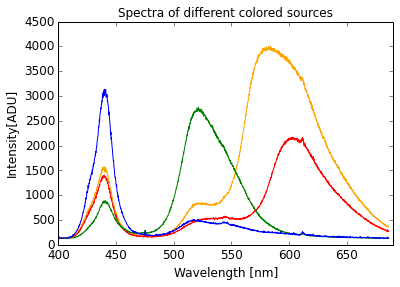
\includegraphics[width=0.5\textwidth]{figures/color}
%Each colored line shows the spectral response to the corresponding color filters. 
\caption{ By adding a color filter in front of a radiating body, we found that the lines peaks around the color's corresponding wavelength in the visible spectrum.The difference in relative intensity is irrelevant, as it may simply be due to how close we are holding the source to the entrance slit of the spectrometer and how much light the colored-marker ink is blocking out. The pixel-to-wavelength conversion was done according to the manufacturer's wavelength calibration coefficients.}
\label{color}
\end{figure}
	\paragraph*{\textbf{Voltage}} The desk lamp is attached to an external potentiometer which allows us to vary the voltage of the source. Since to the relationship between voltage and current is described by Ohm's law, the decrease in voltage is directly proportional to the decrease in current, which  leads to a dimming of the lamp. Another way is to consider the power dissipation by the bulb as described by Eq.\ref{power_ohms}:
	\begin{equation}
	P=IV=\frac{V^2}{R}
	\label{power_ohms}
	\end{equation}
		where P is the power dissipated by the lamp, I is current through the lamp, V is the voltage across the circuit (externally modulated by the potentiometer) and R is the resistance of the circuit which in this case is fixed. Therefore, decreasing the voltage results in a decreases in power dissipation.
		
If we approximate the desklamp source as a radiating blackbody, Wien's law states that its wavelength distribution for different temperature should be approximately the same shape but with a displaced wavelength as shown in Eq.\ref{wien}:
		\begin{equation}
		\lambda_{max} = \frac{b}{T}=\frac{2.897\times 10^3 m\cdot K}{T}
		\label{wien}
		\end{equation}
		where $\lambda_{max}$ is the peak wavelength for the distribution, T is the temperature of the radiating blackbody, and b is the Wien's displacement constant.
		Since Eq. \ref{power_ohms} shows a lower power dissspation for smaller input voltage, it means that the lamp's bulb is cooler in temperature than if it was at a higher voltage setting. This is why the peak wavelength of the  lower-voltage source distribution is longer than the higher-voltage source. % hy the spectra taken with the low voltage setting peaks at a lower wavelength is
	\begin{figure}[h!]
	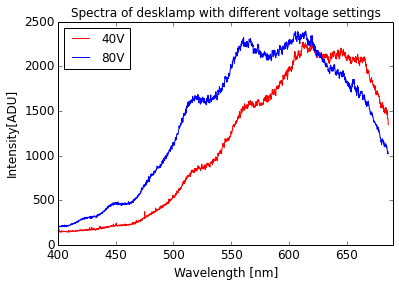
\includegraphics[width=0.5\textwidth]{figures/voltage}
\caption{Changing the input voltage of the source affects the peak wavelength of the distribution. }

\label{voltage}
	\end{figure}
%\subsection{Spectra property and comparison for different sources}
\paragraph*{\textbf{Intensity}}
The sunlight spectra was taken by an optical fiber that lead from spectrometer's entracnce slit to an adjustable stand to minimize the variation of the , however external factors such as cloud and shadows still varied the source brightness. Also,  despite the use of minimum integration time (3ms) for data acquisition,  the pixels still saturate by the high intensity of sunlight as shown in the cutoff in Fig.\ref{sunlight}. Averaging the data does not alleviate the effect since this feature persists throughout the whole duration of taking the 1000 samples. 
 \begin{figure}[h!]
	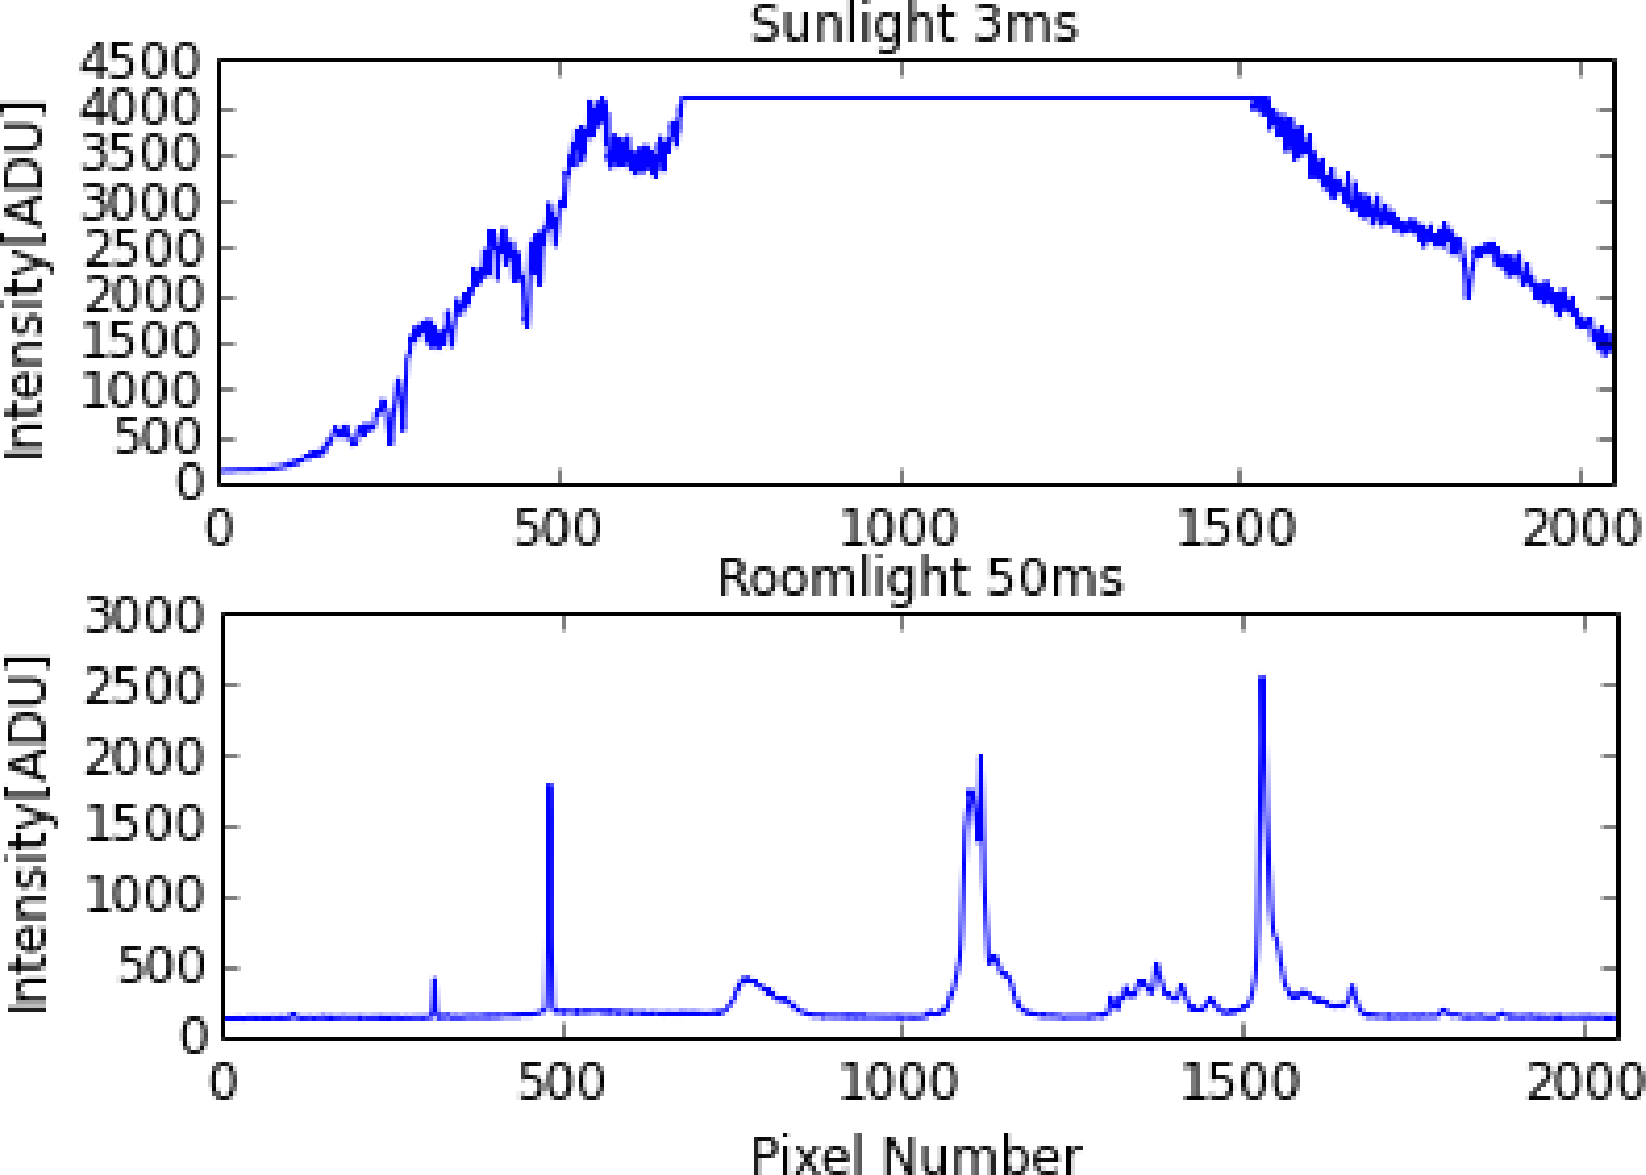
\includegraphics[width=0.45\textwidth]{figures/sunlight_saturated}
\caption{Top: Saturation of the CCD pixels results in the plateau of the spectra. Bottom: Mercury lines in roomlights and spectra obtained from other sources did not exhibit this plateauing effect since none were of such high intensity.}
\label{sunlight}
	\end{figure}
\section{Noise and Systematic Effects}
	 \subsection{Natural Broadening Effect}
 As seen in the mercury lines in Fig.\ref{sunlight}, the spectral lines do not resemble perfectly sharp Dirac Delta functions. This broadening effect is due to several physical phenomena. One reason for  the natural line width is the measurement uncertainty inherent from quantum mechanics. Another more dominant effect is due to the Doppler effect of atoms moving with thermal velocity while they are emitting the electromagnetic wave recorded in the spectra. The distribution of the atomic thermal velocity is governed by the Boltzmann distribution. This Doppler-shifted velocity distribution propagates to our intensity measurement, which can then be rearranged into a Gaussian form. The broadening effect is characterized by the variance of this new distribution.
 \\
\textbf{COMMENT: STOPPED HERE!!!!} 
  \subsection{Dark Counts}
 We took set of 3ms integration time bias frames by placing the red cap on the spectrometer and in a black bag. This integration time was chosen as close to zero as possible to minimize the tails of the Gaussian on the two ends. The 3ms integration time is the shortest integration time accessible for data acquisition using the SpectraSuite software. These dark count measurements can be used to subtract out the per-pixel noise in the experiment's data.
 \begin{figure}[h!]
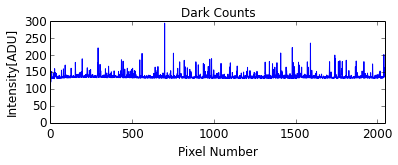
\includegraphics[width=0.5\textwidth]{figures/dark}
\caption{A spectra of neon zoomed in at lower intensity value to show the relative intensity of the signal versus the noise from the dark counts.} 
\label{dark_counts}
\end{figure}
 %A histogram of dark counts is fitted to a Gaussian. 
 %The variance of the distribution relates to the read noise and gain of the spectrometer \citep{ccd_handbook}. 
 \subsection{Poisson nature of obtained data}
 We chose to conduct the statistical analysis on noise property on the 60Watt lightbulb data since the variance is less likely to be dominated by fluctuations in the source's illumination brightness compared to the sunlight or plasma bulb. 
A Gaussian is fitted onto the histogram to obtain the value of mean ($\mu$) and variance($\sigma$) of the distribution. The $\mu$ corresponds to the $ADU_0$, whereas the $\sigma$ corresponds to $\sigma_{ADU_0}$, the error on the dark counts. This variation on the dark counts comes from the non-uniform quality of the pixel as seen in Fig.\ref{dark_counts}. But since $\sigma_{ADU_0}$ is relatively small compared to $ADU_0$, it is negligible when considering its per-pixel additive effect on the raw data.


In real astronomical observations, this method of acquiring dark measurements and the use of overscan strips by adding additional pseudopixels are two common ways of bias calibration on imaging data. Although our spectrometer has a linear CCD array as a detector, imaging telescope often has an plane array of CCD pixels. In those cases, an average of 10 or more bias frame is often better bias-correction technique since it reveals any underlying 2D bias patterns present. 
 \begin{figure}[h!]
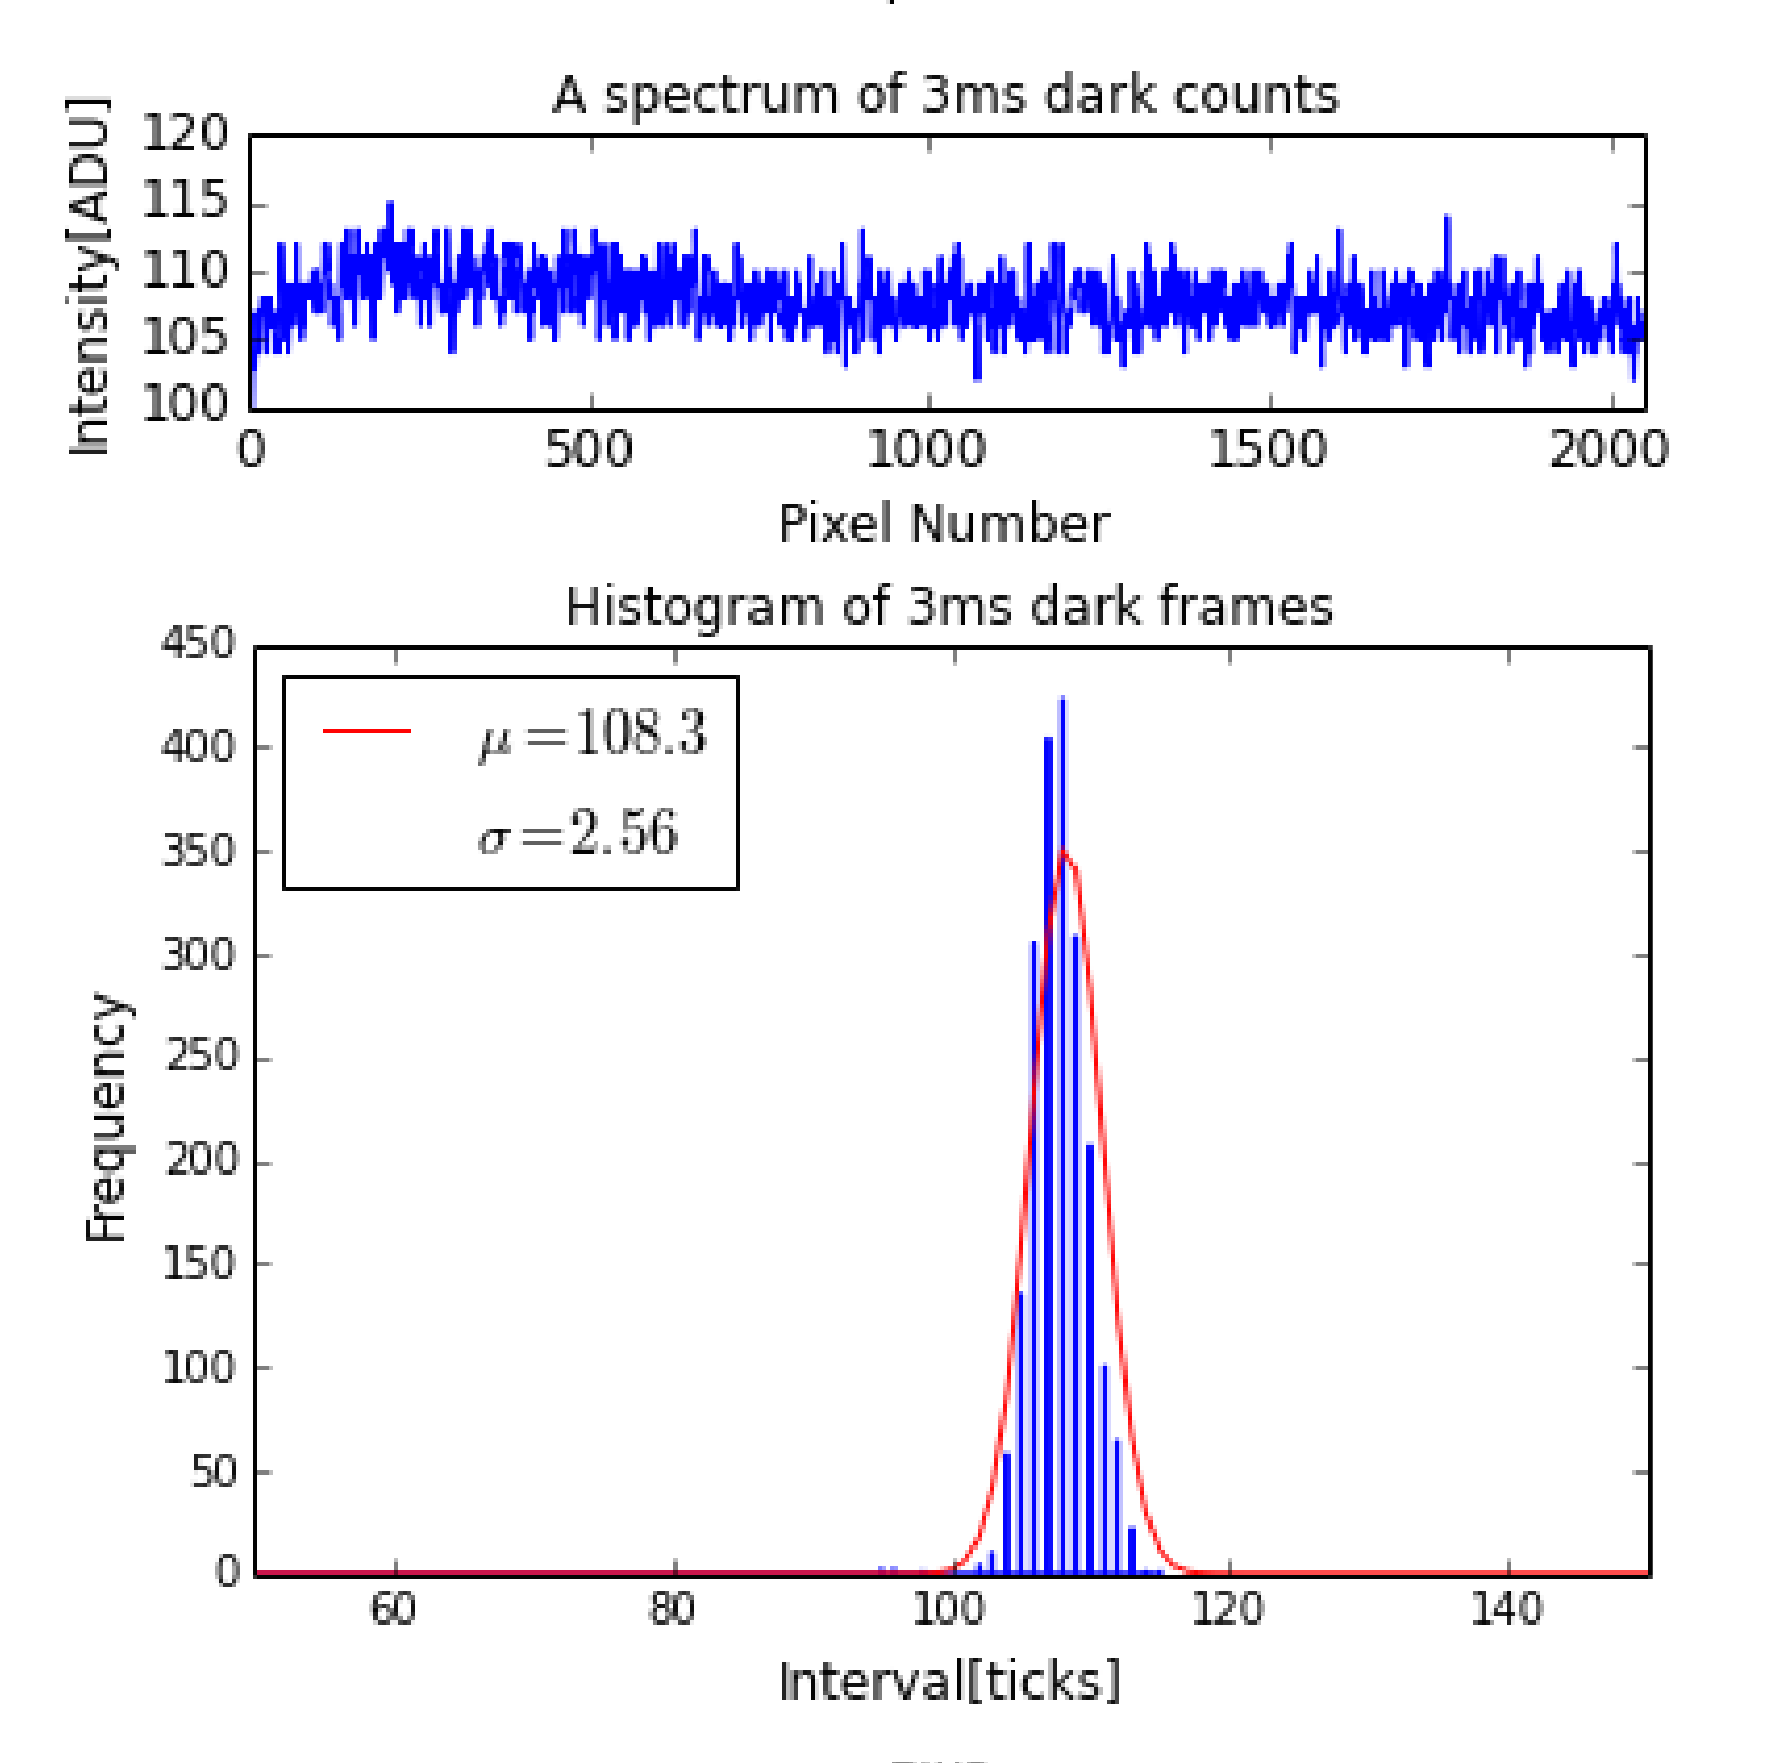
\includegraphics[width=0.45\textwidth]{figures/dark&biashisto}
\caption{Top panel shows an averaged spectra of dark counts that exhibits the non-uniformity of each pixel in the linear CCD array. Also, note the clear bias offset seen at around 125 ADU. Bottom panel is a histogram of bias frames fitted with a Gaussian. } 
\label{dark_counts}
\end{figure}


\subsection{Other possible source of error}
Possible source of error: 
- ununiform pixels(REF dark counts)

Another source of error in our experiment is multiple mixed sources present when taking data. We took preventive measures when taking our data for neon and coarsely covered up the gap between the slit entrance and the neon bulb with its transparent gap removed. This problem could have been completely resolved if data was taken in the dark so that no slight traces of atomic feature of radiating source in the background can be seen in the pure neon sample used for wavelength calibration.
\section{Data Reduction}
 Now we have examined the systematic effects that affects our data, we process the raw data obtained from the spectrometer in order to find an equation that converts the pixel values to wavelengths.
  \subsection{Data Smoothing}
  Smoothing is a data reduction technique that removes noise and minor pixel-to-pixel variations in the data. We employ both the boxcar and averaging technique in our datasets and compare their resulting differences.
  \paragraph*{\textbf{Boxcar Smoothing}}
  Our boxcar smoothing algorithm takes the values of adjacent pixel and average them over some user-defined interval. Since the quality of each pixel is inconsistent, boxcar smoothing compensate for the pixel-by-pixel variations.  However even though boxcar smoothing lowers the signal-to-noise ratio by eliminating small-scale features, it also lowers the resolution of the Delta-function-like peak that are important spectral features. Dataset processed in such manner has adverse effects on centroid value calculation shown in Fig.\ref{boxcar} when the interval is chose incorrectly.
 \begin{figure}[h!] 
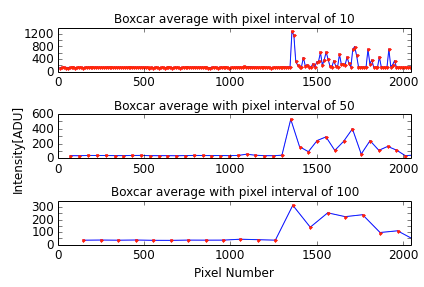
\includegraphics[width=0.45\textwidth]{figures/boxcar}
\caption{The red marker denotes the interval that we are averaging over. As the number of pixels in an averaging interval increases, the shape of the line and the location of its extrema is obscured by the lack of datapoints defining it.}\label{boxcar}
\end{figure}
 \paragraph*{\textbf{Average multiple spectra samples}}
Since the boxcar method produced undesirable results, we resorted to the conventional averaging of data by summing over the intensity values of each pixel of the same experiment then scaling the result by the number of datasets. This is a step towards finding a functional form to fit the data since it makes the data less discrete and more continuous like a function. 
	\subsection{Centroid-Finding Methods}
	\paragraph*{\textbf{Automated centroid algorithm}}
 We attempted to create an automated centroid algorithm by imposing two conditions to select for the centroid of interest that correspond to atomic signature spectral lines. The selected data range used for centroid calculation must begin at a local minimum and contain one local maximum and then end with another local minimum. There can not be any extra extrema that lies within that range other than the 3 specified. Since a large number of datapoints satisfies this condition, we needed a quantitative measure of how ``important" the spike is.  
 
 For this, we use the intensity difference between the consecutive  local maximum and minimum and select only the data ranges that  have  differences greater than 10\% of the difference between the absolute maximum and  minimum datapoint of the whole dataset. The ad hoc 10\% criterium was chosen to so that the bias offset  was considered in . The 10\% was chosen because of the quality of the centroid result that it produces. The local extrema was found by comparing consecutive data points and testing a change in the boolean condition of increasing or decreasing.
\begin{figure}
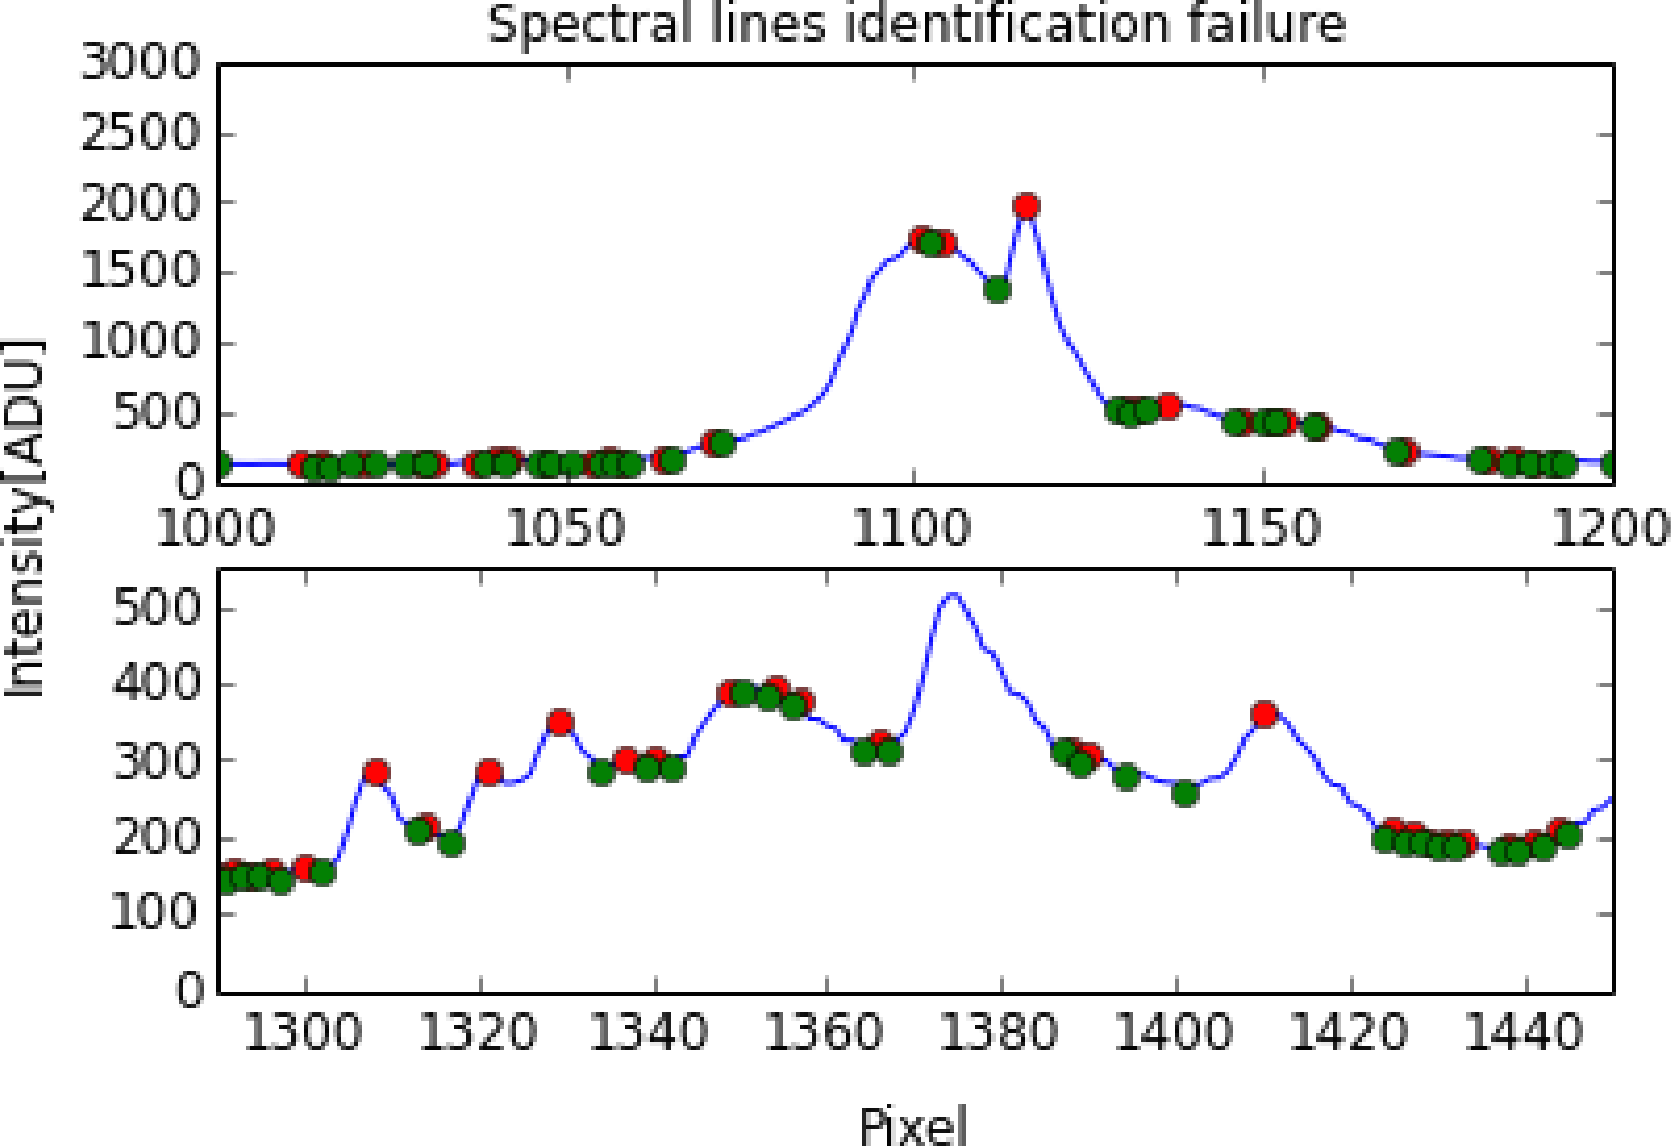
\includegraphics[width=0.45\textwidth]{figures/fail}
\caption{Top: The closely spaced extremum at around the 1100th pixel results in a small difference value between the local minimum and maximum. Therefore, it was not detected by the algorithm. Bottom: The extremum finding algorithm did not detect the maximum at around pixel 1380 in its  first step.}
\end{figure}


	The algorithm was not very robust as it is unable pick out spectral lines that lied between consecutive extrema, such as the ones near pixel 1115 and 1374 in Fig.\ref{fail}. Despite the attempts to vary the percentage cut, the program cannot identify features that showed relative differences, so it tends to overlook single, short, sharp spikes. The variability in the importance of a signature line  is hard to account for  by measuring only the  absolute differences.
\begin{figure}
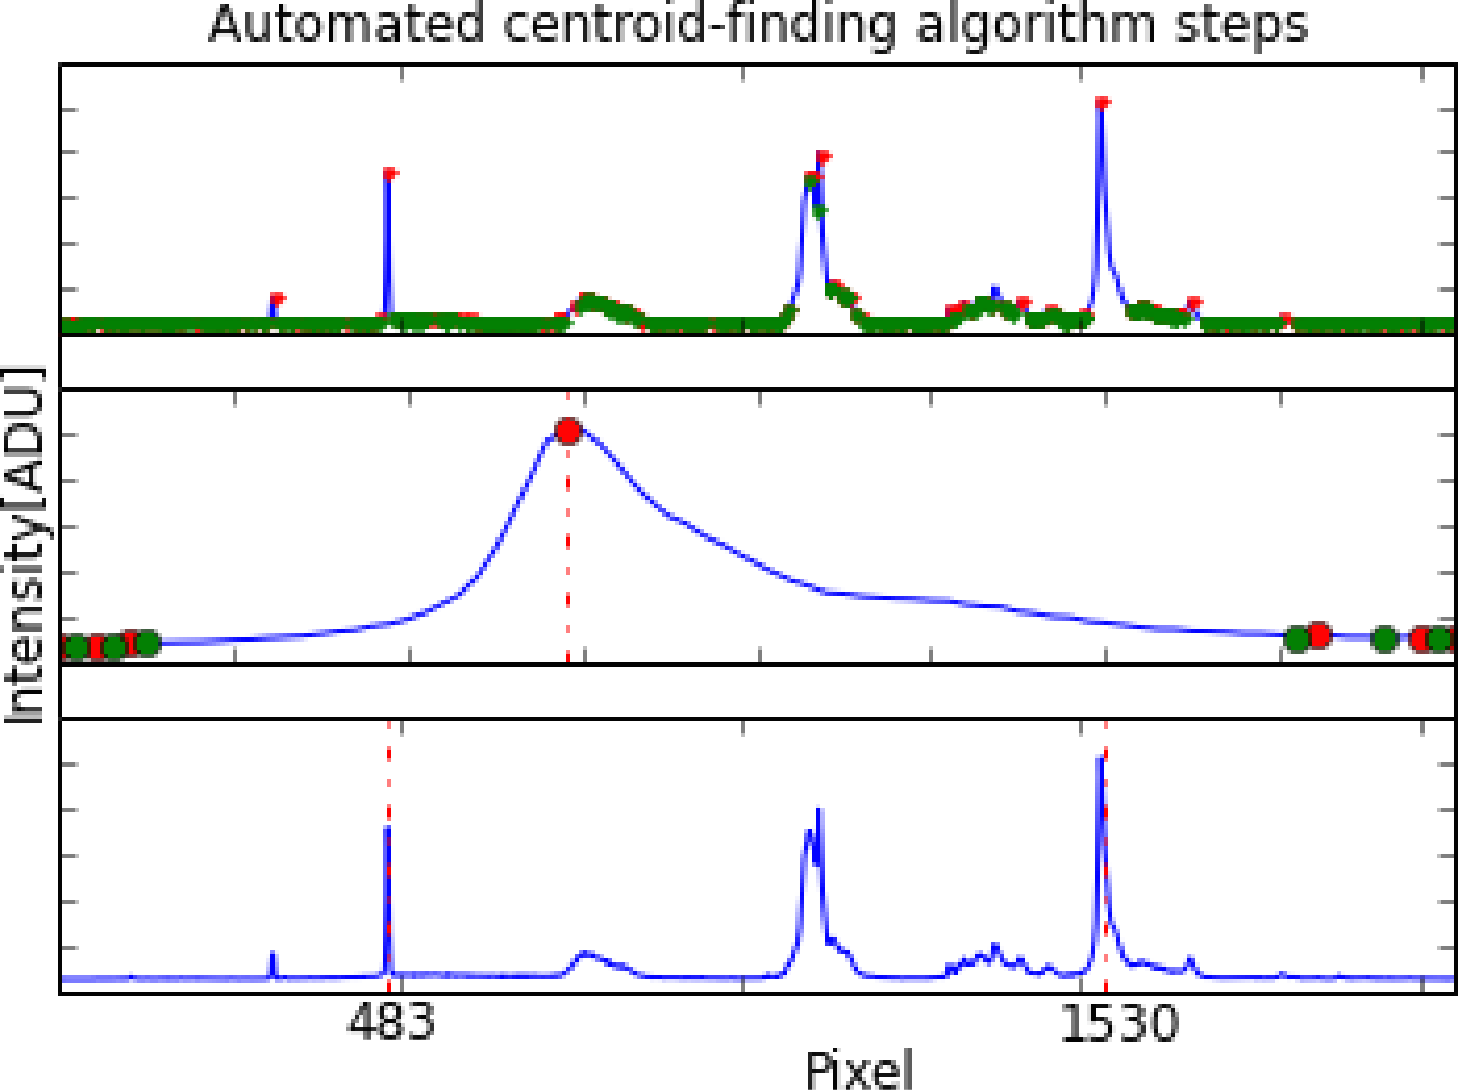
\includegraphics[width=0.45\textwidth]{figures/steps}
\caption{Graphical representation of how the automated algorithm works. Top: Identifying all the extremum of the dataset. Red marker denotes local maximum; green denotes local minimum. Middle: Applying criteria to select suitable ranges as shown in middle plot, using this sliced dataset to obtain the centroid values (dashed). Bottom: Resulting centroid list misses some important spectral feature picked out by the estimation method  described in Sec.\ref{estimate}.}\label{fail}
\end{figure}
\paragraph*{\textbf{Estimation method}} 
Since we can approximate the shape of a single atomic line feature as a Gaussian with the data range is isolated, plus-or-minus one sigma accounts for about 68\% of the area under a Gaussian.
we manually select data range. then 
\label{estimate}
\subsection{Wavelength calibration}
The polynomial nature of our fitting model comes from a diffraction scenario, in which $----$. The  small angle approximation results in a Taylor expansion that can be boiled down to a polynomial of higher order terms. In this case, the fitting parameter is the polynomial coefficients The residual is defined as $y_i-f(x_i)$ where $y_i$ is the centroid value in pixels from experimental result and f is the polynomial fitting model.  We plot the residual in order to examine whether  there are any patterns present in the residual which would suggest a need for a higher order fit.
\begin{figure}
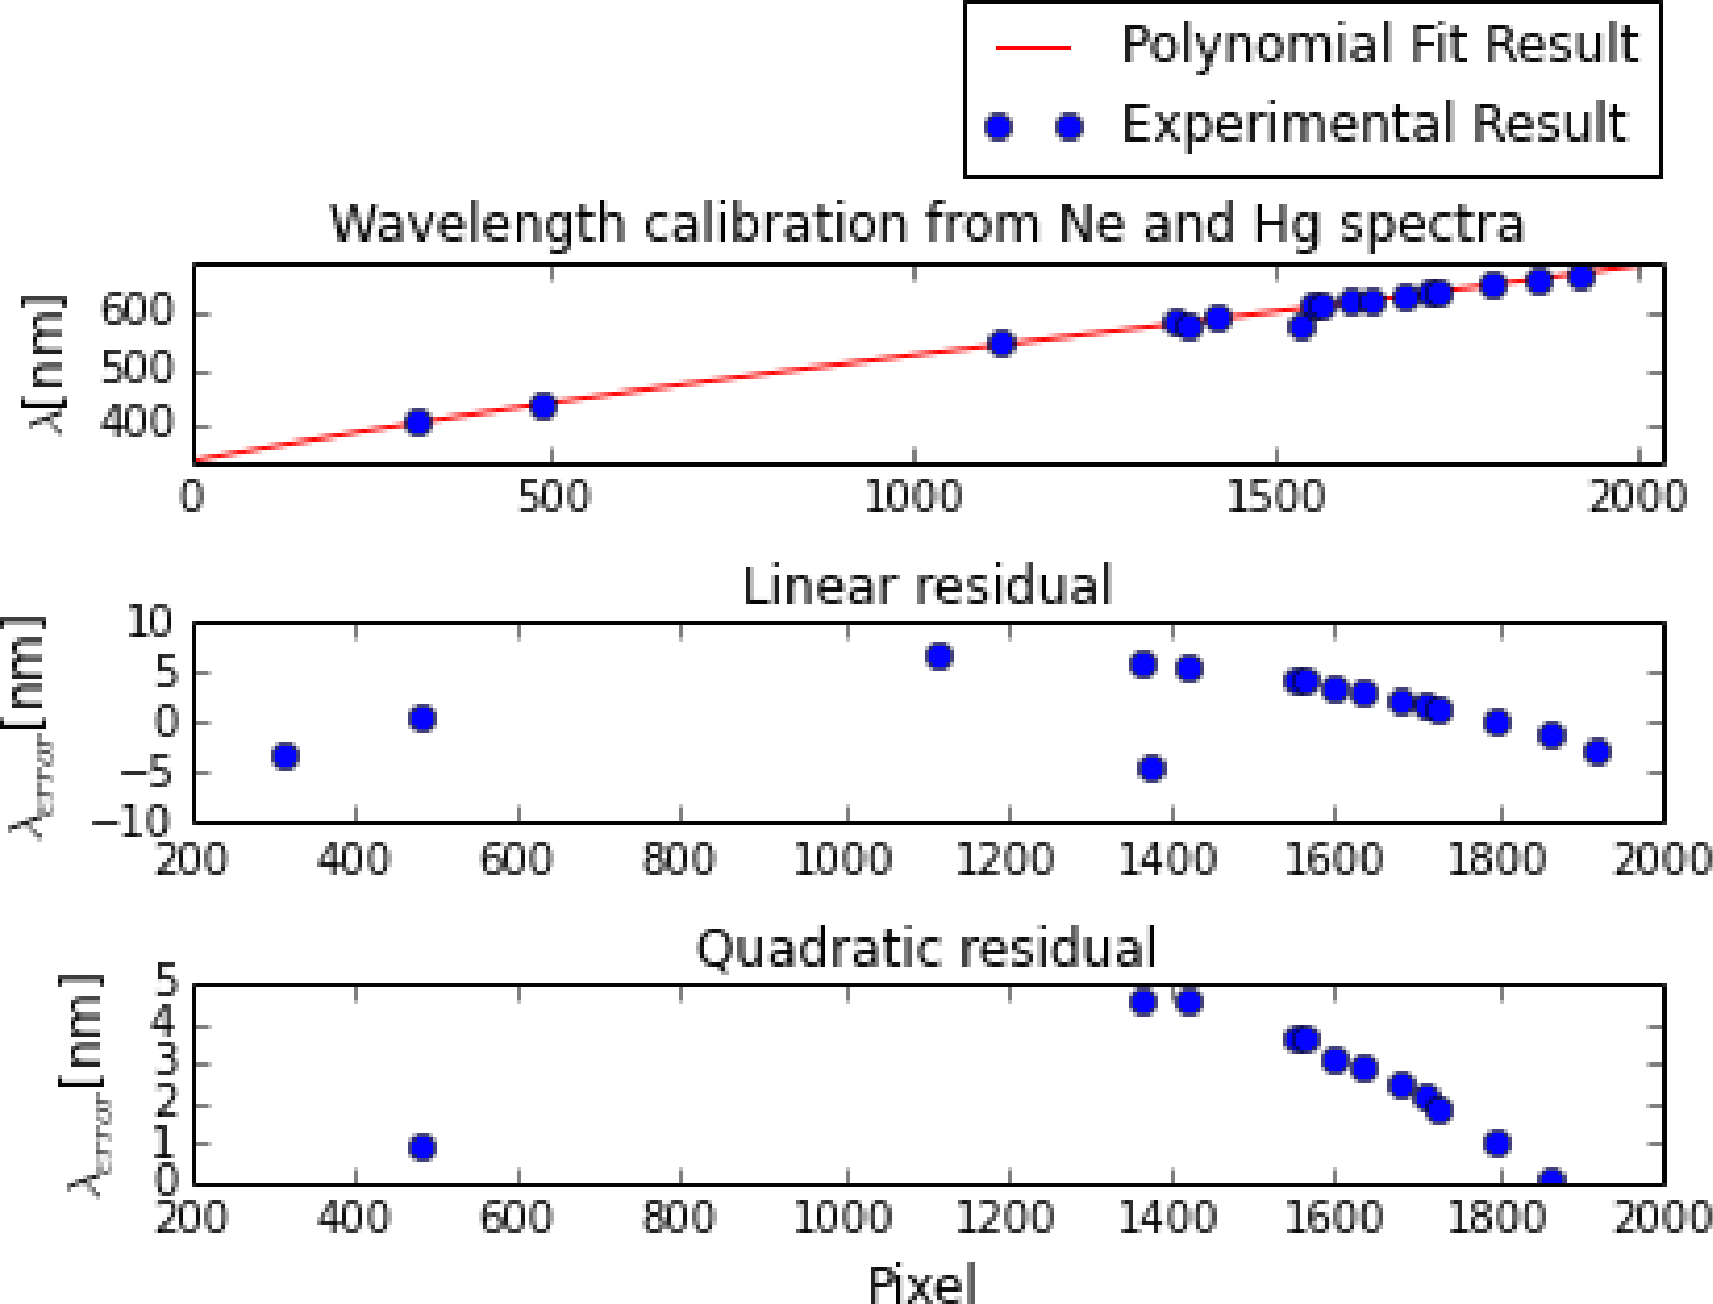
\includegraphics[width=0.5\textwidth]{figures/neon_calib}
\caption{Top panel shows the result of a linear least square fit on the centroid values obtained from the neon and mercury spectra. The middle and bottom panel is residual plot from comparing against the linear and quadratic fits respectively.}\label{neon_calib}
\end{figure}
\begin{figure}
\label{comp_linquad}
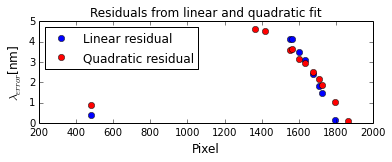
\includegraphics[width=0.5\textwidth]{figures/compare_linquad}
\caption{Above is an overlaid plot of the linear and quadratic residuals. It shows that there is not much improvement in using a higher order polynomial model than the linear one. This makes sense because the polynomial coefficient that we obtained for the quadratic term is $-5.101\times 10^{-6}$, which is an order of magnitude smaller than the quadratic coefficient in the manufacturer's wavelength calibration. This is the reason why the y-axis range of the linear residual plot in Fig.\ref{neon_calib} is almost the same as the range in the quadratic residual plot.} 
\end{figure}
\section{Conclusion}
In this experiment, we measured the effect of different light-emitting sources to 
Possible extension to this project may be to try conducting a basic flat-field correction to the detector. One way to do this to shine bright light uniformly on the detector to see the response of each pixel. The exposure time needs to be short so that the CCD is not saturated. We can also try to measure maximum ranges at which CCD is sensitive and linear.
\section{References}
%\bibliographystyle{elsarticle-harv}
\begin{itemize}
\item Howell, Steve,  \textit{Handbook of CCD Astronomy}, 2nd Edition. Cambridge University Press, 2006.
\item Haken, Hermann and Wolf, Hans Christolph, \textit{The Physics of Atoms and Quanta}, Springer-Verlag, 1996.
\item Tipler, Paul and Llewellyn, \textit{Modern Physics}, Macmillan, 2012.
\item Hecht, Eugene, \textit{Optics}, Addison-Wesley, 2001.
\end{itemize}
\end{document}
